Agora que sabemos como criar uma gema, visto no capítulo \ref{chapter:criacao_de_bibliotecas_do_ruby},
podemos partir para a ideia de fazer modificações em uma gema que já existe, ou seja, fazer a
adaptação de uma gema, adicionando novas funcionalidade.

Suponha o cenário aonde utilizamos com frequência uma certa gema, no entanto apesar dela comportar várias 
funcionalidades, ela não possui tudo que desejamos. Neste caso, basta fazer a adaptação desta gema, não 
sendo necessário criar uma nova gema do zero.

É válido verificar se a funcionalidade que esteamos adicionando, esta no mesmo contexto da gema.
Pois por exemplo, se estamos utilizando uma gema matemática e ela não possuir uma função para calcular a 
raiz de um número, podemos fazer uma modificação nesta gema para que ela possa calcular a raiz. 
Por outro lado, não faz nenhum sentido incluuir uma funcionalidade de criar mapas do \emph{Google}, pois 
esta funcionalidade não está no mesmo contexto da gema.

Para facilitar o entendimento utilizaremos para a explicação a gema 
\emph{\href{https://github.com/toshikomura/Google-Maps-for-Rails}{Google-Maps-for-Rails}} 
\footnote{Google-Maps-for-Rails : \url{https://github.com/toshikomura/Google-Maps-for-Rails}} que é um 
\emph{branch} da gema 
\emph{\href{https://github.com/apneadiving/Google-Maps-for-Rails}{Google-Maps-for-Rails}} 
\footnote{Google-Maps-for-Rails : \url{https://github.com/apneadiving/Google-Maps-for-Rails}} criada por 
\emph{\href{https://github.com/apneadiving}{Benjamin Roth}} 
\footnote{Bejamin Roth: \url{https://github.com/apneadiving}} e 
\emph{\href{https://github.com/MrRuru}{David Ruyer}} \footnote{David Ruyer: \url{https://github.com/MrRuru}}.

Essa gema criada por \emph{Bejamin Roth} e \emph{David Ruyer} tem como objetivo criar mapas de forma 
simplificada, proporcionando a inclusão de sobreposições oferecidas pelo \emph{Google}, como por exemplo,
marcadores e circulos. Ela também possui um código bem flexível que permite a aceitação de outros 
provedores de mapas, como por exemplo o \emph{Bing Maps} [\citeonline{google_maps_for_rails}].

Este capítulo tem o objetivo de mostrar os passos que devem ser realizados para se adaptar uma biblioteca
do \emph{Ruby}. Na seção \ref{section:engenharia_reversa}, apresentaramos o processo de engenharia
reversa para gerar diagramas que representam o sistema em um alto nível de abstração, sendo seguida pela
seção \ref{section:entendimento_da_biblioteca_do_ruby}, onde apresentaramos como fazer a leitura dos diagramas de alto
nível. depois na seção \ref{section:adaptações}, mostraremos o processo de adaptação e os cuidados que devemos
tomar, e fecharemos o capítulo com a seção \ref{section:exemplo_de_uso_de_google-maps-for-rails}, onde
apresentaramos o uso da gema de exemplo que adaptamos. Caso haja interesse, também pode-se consultar o
apêndice \ref{chapter:api_do_google_maps} para conhecer um pouco da história e da \emph{API} do
\emph{Google Maps}.

\section{Engenharia Reversa}
\label{section:engenharia_reversa}

Esta seção tem o objetivo de apresentar a importância da \emph{engenharia reversa} no processo de adaptação
de uma gema. Inicialmente veremos uma definição do processo de \emph{engenharia reversa} e depois
apresentaremos este processo sendo realizado na gema \emph{Google-Maps-For-Rails}.

Para conseguirmos entender o funcionamento de uma gema, precisamos obrigatoriamente fazer uma tradução
do código fonte para diagramas, pois não conseguiremos fazer nenhuma modificação consistente
se não tivermos uma visão geral de seu funcionamento, e esse procedimento de tradução se chama 
\emph{engenharia reversa}.

\emph{Engenharia reversa} é um processo de análise para a extração de informações de algo que já 
existe em um modelo de abstração de alto nível. Essas informações podem estar no formato de código 
fonte ou mesmo em um executável. O processo de análise para a extração de dados deve ser feita de forma
minunciosa, pois pode ocorrer uma grande perda de recursos, caso alguma funcionalidade seja entendida de
forma incorreta. E o modelo de abstração de alto nível, pode ser por exemplo um diagrama de caso de uso ou
um diagrama de sequência.

Aplicando a \emph{engenharia reversa} na gema \emph{Google-Maps-For-Rails} conseguimos obter como resultado:
o diagrama de classe na imagem \ref{fig:diagrama_de_classes_google_maps_for_rails}, o diagrama de
atributos na imagem \ref{fig:diagrama_de_atributos_google_maps_for_rails} e o diagrama de herança na
imagem \ref{fig:diagrama_de_heranca_google_maps_for_rails}, que serão explicados em mais detalhes logo a
seguir.

Nenhum dos 3 diagramas segue os seus respectivos padrões, isso se deve ao fato de que não existia espaço 
suficiente na imagem para representar o sistema da gema por completo. Por esse motivo optamos por definir 
novos diagramas que possuem características sinilares aos seus padrões, mas com algumas características
adicionais.

Para as imagens de diagrama de classes na imagem \ref{fig:diagrama_de_classes_google_maps_for_rails} e
o diagrama de atributos na imagem \ref{fig:diagrama_de_atributos_google_maps_for_rails} as seguintes
explicações são válidas:

\begin{itemize}

 \item Cada retângulo representa uma classe da gema.
 
 \item O nome ácima dos traços ‘‘-----'' representa o nome da classe.
 
\begin{comment} 
 
 \item O símbolo ‘‘*'' do lado esquerdo do nome da classe representa que ela é \emph{superclasse} e o 
 símbolo ‘‘*'' do lado direito do nome da classe representa que ela é uma \emph{subclasse}, por exemplo
 ‘‘\emph{* Objects.BaseBuilder}'' é \emph{superclasse} de ‘‘\emph{Google.Builders.Map *}'', neste caso 
 ‘‘\emph{Google.Builders.Map *}'' é \emph{subclasse} de ‘‘\emph{* Objects.BaseBuilder}''. O mesmo 
 critério é válido para o símbolo ‘‘\$''.
 
 \item O símbolo ‘‘+'' do lado esquerdo do nome da classe representa que ela é \emph{incluída} em outra  
 \emph{classe} e o símbolo ‘‘+'' do lado direito do nome da classe representa que ela \emph{incluí} outra 
 \emph{classe}, por exemplo ‘‘\emph{+ Google.Objects.Common}'' é \emph{incluída} na \emph{classe} 
 ‘‘\emph{Google.Objects.Bound \$+}'', neste caso ‘‘\emph{Google.Objects.Bound \$+}'' \emph{incluí} a 
 \emph{classe} ‘‘\emph{+ Google.Objects.Common}''.
 
\end{comment}

 
\end{itemize}

\begin{figure}[ht]
  \begin{center}     
    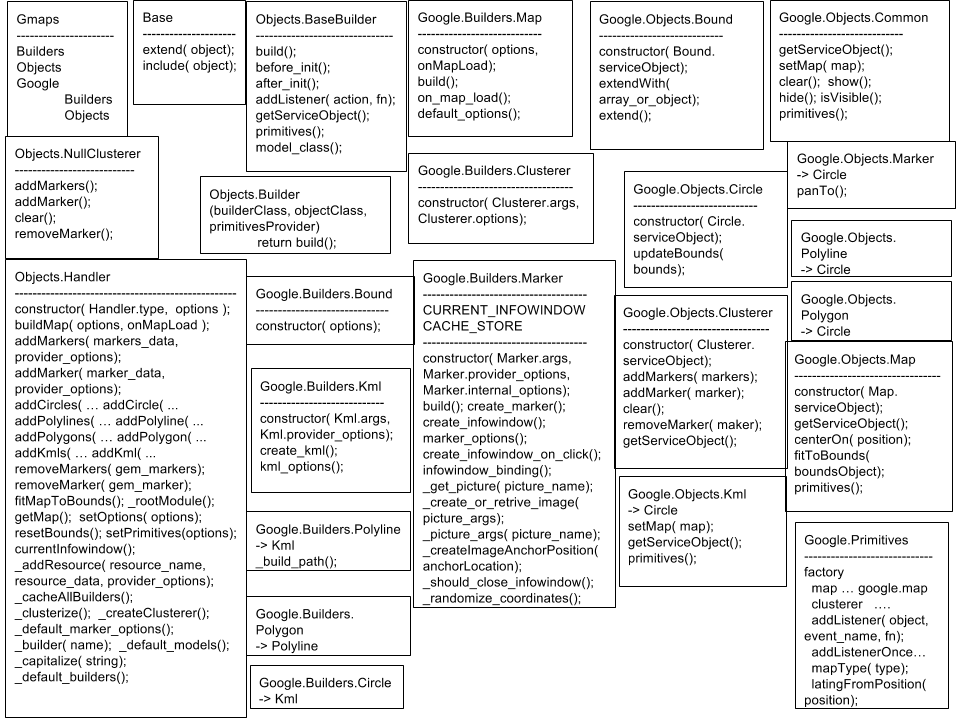
\includegraphics[scale=0.35]{images/diagrama_de_classes_google_maps_for_rails.png}
    \caption{Diagrama de Classes Google-Maps-For-Rails}
    \label{fig:diagrama_de_classes_google_maps_for_rails}
  \end{center}
\end{figure}

\begin{comment}
Percebe-se que o diagrama de classe na imagem ‘‘Figure \ref{fig:diagrama_de_classes_google_maps_for_rails} - 
Diagrama de Classes Google-Maps-For-Rails'' não segue os padrões de um diagrama de classes, por causa que 
no espaço disponível na imagem não seria possível inserir o sistema por completo, comprometendo o 
entendimento da gema. Por esse motivo as definições deste diagrama serão explicados logo a seguir.
\end{comment}

As seguintes explicações são válidas para o diagrama de classe na imagem
\ref{fig:diagrama_de_classes_google_maps_for_rails}:

\begin{itemize}

 \item O digrama não mostra os atributos das classes. 
 
 \item Todos os nomes seguidos de ‘‘(...)'' abiaxo do traço ‘‘-----'' representam os métodos da classe.
 
 \item Existem classes que não possuem os traços ‘‘-----'', neste caso elas possuem o nome delas
 seguida do símbolo ‘‘->'' e depois um nome de outra classe. Isso significa que esta classe
 possui os mesmo métodos da classe que vem depois do símbolo ‘‘->''. Por exemplo a 
 classe ‘‘\emph{Google.Builder.Circle -> Kml}'' representa a classe ‘‘\emph{Google.Builder.Circle}'' 
 e ela possuí os mesmo métodos da classe ‘‘\emph{Kml}'', ou seja, ela possuí os métodos
 ‘‘\emph{constructor()}'', ‘‘\emph{create\_...()}'' e ‘‘\emph{...\_option()}''. E também existe o caso 
 onde esta classe possuí métodos além dos da outra, e neesse caso esses métodos são colocados na linha 
 de baixo. Por exemplo a classe ‘‘\emph{Google.Builder.Polyline -> Kml}'' que é a classe 
 ‘‘\emph{Google.Builder.Polyline}'', além de possuír os métodos da classe \emph{Kml}, ela 
 possuí o método ‘‘\emph{\_build\_path()}''.
 
\end{itemize}

\begin{figure}[ht]
  \begin{center}     
    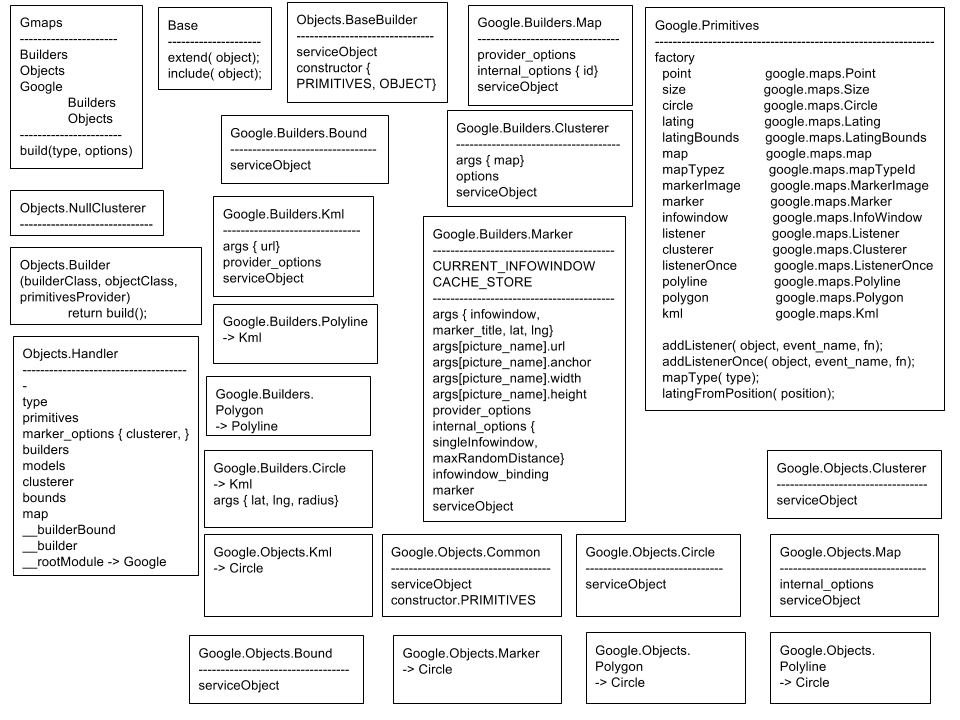
\includegraphics[scale=0.35]{images/diagrama_de_atributos_google_maps_for_rails.png}
    \caption{Diagrama de Atributos Google-Maps-For-Rails}
    \label{fig:diagrama_de_atributos_google_maps_for_rails}
  \end{center}
\end{figure}

\begin{comment}
O diagrama de atributos na imagem ‘‘Figure \ref{fig:diagrama_de_atributos_google_maps_for_rails} - 
Diagrama de Atributos Google-Maps-For-Rails'' não é um diagrama padrão de projeto, mas neste caso ele
serve como complemento do diagrama de classe ‘‘Figure \ref{fig:diagrama_de_classes_google_maps_for_rails} - 
Diagrama de Classes Google-Maps-For-Rails'', e isso também foi feito por causa do pouco
espaço disponível na imagem. Por esse motivo as definições deste diagrama serão explicados logo a seguir.
\end{comment}

As seguintes explicações são válidas para o diagrama de atributos apresentado na imagem
\ref{fig:diagrama_de_atributos_google_maps_for_rails}:

\begin{itemize}
 
 \item Todos os nomes abiaxo do traço ‘‘-----'' representam os atributos da classe. Também 
 existe o caso onde esse métodos são seguidos pelos símbolos ‘‘\{ ... \}'', onde o método é um 
 \emph{objeto} e os nomes separados por ‘‘,'' entre os símbolos ‘‘\{ ... \}'' são os atributos
 do \emph{objeto}.
 
 \item Existem classes que não possuem os traços ‘‘-----'', neste caso elas possuem o nome delas
 seguida do símbolo ‘‘->'' e depois um nome de outra classe. Isso significa que esta classe 
 possui os mesmo atributos da classe que vem depois do símbolo ‘‘->''. Por exemplo a 
 classe ‘‘\emph{Google.Builder.Polyline -> Kml}'' que representa a classe 
 ‘‘\emph{Google.Builder.Polyline}'', ela possuí os mesmo atributos da classe
 ‘‘\emph{Kml}'', ou seja, ela possuí os atributos 
 ‘‘\emph{args \{ url \}}'', ‘‘\emph{provider\_option}'' e ‘‘\emph{serviceObject}''. E também existe o caso 
 onde esta classe possuí atributos além dos da outra classe e neesse caso esses 
 atributos são colocados na linha de baixo. Por exemplo a classe 
 ‘‘\emph{Google.Builder.Circle -> Kml}'' que é a classe ‘‘\emph{Google.Builder.Circle}'', além de 
 possuír os atributos da classe \emph{Kml}, ela possuí o atributo 
 ‘‘\emph{args \{ lat, lng, radius \}}''.
 
\end{itemize}

\begin{figure}[ht]
  \begin{center}     
    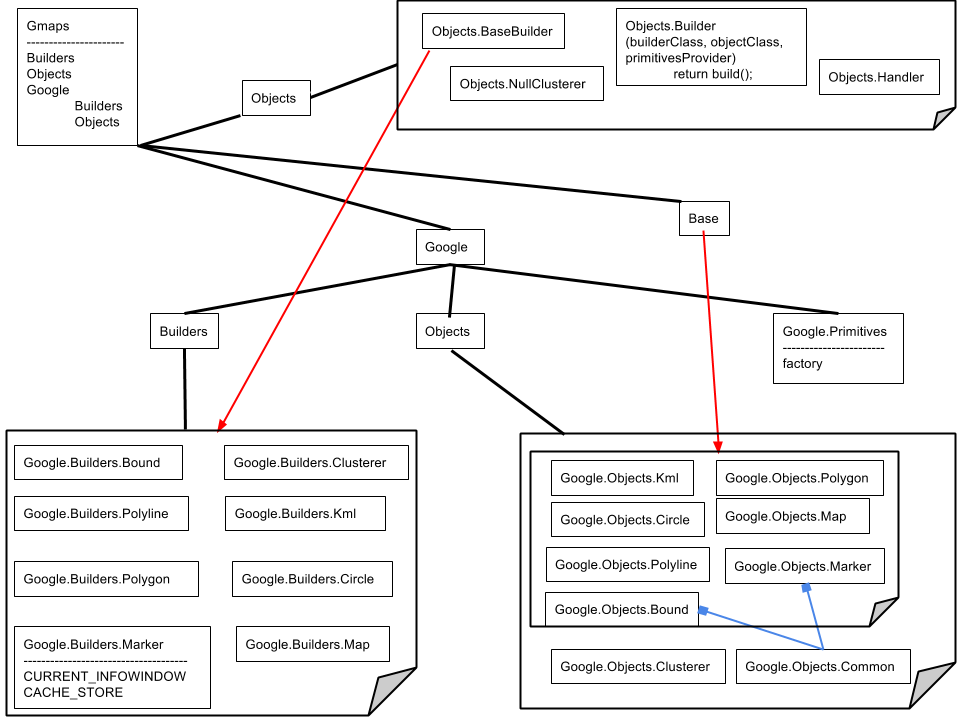
\includegraphics[scale=0.35]{images/diagrama_de_heranca_google_maps_for_rails.png}
    \caption{Diagrama de Herança Google-Maps-For-Rails}
   \label{fig:diagrama_de_heranca_google_maps_for_rails}
  \end{center}
\end{figure}

\begin{comment}
O diagrama de herança na imagem ‘‘Figure \ref{fig:diagrama_de_heranca_google_maps_for_rails} - 
Diagrama de Herança Google-Maps-For-Rails'' não é um diagrama padrão de projeto, mas neste caso ele também
serve como complemento do diagrama de classe ‘‘Figure \ref{fig:diagrama_de_classes_google_maps_for_rails} - 
Diagrama de Classes Google-Maps-For-Rails'', e isso também foi feito por causa do pouco
espaço disponível na imagem. Por esse motivo as definições deste diagrama serão explicados logo a seguir.
\end{comment}

As seguintes explicações são válidas para o diagrama de herança na imagem
\ref{fig:diagrama_de_heranca_google_maps_for_rails}:

\begin{itemize}

 \item As linhas pretas indicam a organização da gema sendo que a classe \emph{Gmaps} é a classe principal.
 
 \item Os retângulos normais representam as classes.
 
 \item A classe \emph{Gmaps} possui os atributos \emph{Builders}, \emph{Objects} e 
 \emph{Google}, onde o \emph{Google} possui os atributos \emph{Builders} e \emph{Objects}.
 
 \item As linhas vermelhas com pontas de seta representam a herança entre duas \emph{classes}, onde 
 a classe que está com a seta, é a classe que herda as características da classe
 na outra ponta da linha.

 \item As linhas azuis com pontas de quadrado representam a inclusão de uma classe na outra, onde
 a classe que está com o quadrado, é a classe que incluí a classe que está na outra ponta da linha.
 
  \item Os retângulos que tem uma dobra no canto inferior direito representam um conjunto de classes, 
 onde estas classes possuem uma característica em comum. Por exemplo as classes ‘‘\emph{Kml}'', 
 ‘‘\emph{Polygon}'', ‘‘\emph{Polyline}'', ‘‘\emph{Circle}'', ‘‘\emph{Map}'', ‘‘\emph{Marker}'' e 
 ‘‘\emph{Bound}'' que são ‘‘\emph{Objects}'' do ‘‘\emph{Google}'', estão em um conjunto onde todas elas 
 herdam as características da classe ‘‘\emph{Base}''.
 
 \end{itemize}
 
 
\section{Entendimento da Biblioteca do Ruby} 
\label{section:entendimento_da_biblioteca_do_ruby} 

Agora que realizamos a \emph{engenharia reversa} da \emph{gema} para construidos os diagramas
de alto nível na seção anterior \ref{section:engenharia_reversa}. Podemos apresentar
nesta seção, a análise de algumas características dos diagramas, respondendo à algumas perguntas,
como por exemplo:

\begin{itemize}

 \item Qaais as principais classes da gema ?
 
 \item Quais são as classes mais usadas na gema ?
 
 \item Quais são as classes de controle da gema ?
 
 \item A gema possui classes de configuração ? Quais são elas ?
 
\end{itemize}

Para a gema de exemplo, encontramos as seguinte características que serão listadas e explicadas
logo a seguir.

\begin{itemize}

 \item Apesar do ‘‘\emph{GMaps}'' ser a classe principal da gema, ela não é a mais
 importante, pois todas as funcionalidades da gema são controladas pela classe
 ‘‘\emph{Hanlder}''. A única funcionalidade da classe ‘‘\emph{GMaps}'' é fazer a chamada
 para a criação de ‘‘\emph{Handler}'', ou seja quando se requisita o método 
 ‘‘\emph{GMaps.build('Google')}'' o método verifica se o objeto ‘‘\emph{Handler}'' já
 existe, e caso ele não exista, o ‘‘\emph{GMaps}'' faz a criação chamando o método 
 ‘‘\emph{new Gmaps.Objects.Handler(type, options)}''.

 \item ‘‘\emph{Hander}'' é a classe que controla todo o funcionamento da gema e 
 basicamente ela possui dois momentos:
 
  \subitem - No primeiro momento ela prepara a estrutura da \emph{gema} para criação e manipulação
  do mapa, criando e setando os objetos de configuração, como por exemplo criando o \emph{objeto}
  ‘‘\emph{Primitives}''.
  
  \subitem - No segundo momento ela cria o mapa com as configurações e permite a manipulação do mapa, 
  possibilitando a criação e inserção de sobreposições como \emph{circles} e \emph{polylines}.
 
 \item A classe ‘‘\emph{Primitives}'' possui as definições que são comuns na gema, 
 como por exemplo, é ela possui a definição do tipo ‘‘\emph{Marker: google.maps.Marker}'' que 
 é a classe \emph{Marker} do \emph{Google Maps}.
 
 \item O atributo ‘‘\emph{serviceObject}'' de todas as classes de 
 ‘‘\emph{Builders}'' do ‘‘\emph{Google}'', representam o atributo que recebe o objeto do 
 \emph{Google Maps}.
 
\end{itemize}
 
\section{Adaptações}
\label{section:adaptações}

Esta seção tem o objetivo de mostrar como podemos fazer adapatações em gemas, após realizar o processo de
\emph{engenharia reversa} e o processo de entendimento da gema. Inicialmente veremos quais os objetos que
precisam ser incluídos, depois quais funcionalidades adicionais são necessárias, e por fim, analisaremos o
quanto essas modificações afetaram o funcionamento original da gema.

Tendo a abstração de alto nível para a gema \emph{Google-Maps-For-Rails}, podemos partir para a 
adaptação dela, ou seja, agora que temos alguns diagramas que nos auxiliam a visualizar o funcionamento 
geral da gema, podemos tentar acrescentar novas funcionalidades, analisando os locais das possíveis 
modificações e os impactos que essas mudanças podem causar. 

A gema já possuí sobreposições como \emph{markers} e \emph{circles}, mas até o momento não possuí a 
funcinalidade de criar direções entre um ponto de origem e um ponto de destino. Contudo a ideia é criar 
uma funcionalidade que receba como parâmetro um local de origem e um local de destino, e retorne como
resultado uma sequência de ruas e direções a serem seguidas para ir do local de origem ao local de destino.

Para realizarmos essa modificação foi necessário consultar a \emph{API} do 
\emph{\href{https://developers.google.com/maps/documentation/javascript/directions}{Direction Service}} 
\footnote{Direction Service: \url{https://developers.google.com/maps/documentation/javascript/directions}}
(\emph{Serviço de Direção}) do \emph{Google}, onde verificamos que seria necessário o uso de pelo menos
quatro \emph{classes} que serão listadas e explicadas logo a seguir:

\begin{itemize}

 \item ‘‘\emph{DirectionService}'' (\emph{google.maps.DirectionsService}) é a classe que tem o 
 objetivo de requisitar e receber o caminho entre o local de origem e o local de destino.
 
 \item ‘‘\emph{DirectionRender}'' (\emph{google.maps.DirectionsRenderer}) é a classe que tem o 
 objetivo de rederizar no mapa o caminho, entre o local de origem e o local de destino.
 
 \item ‘‘\emph{TravelMode}'' (\emph{google.maps.TravelMode}) é a classe que tem o objetivo de 
 informar a forma como esse caminho deve ser percorrido, que pode ser caminhando (walking), de carro 
 (driving), bicicleta (bicycling) e/ou por meios de locomoção públicos (transit).
 
 \item ‘‘\emph{DirectionsStatus}'' (\emph{google.maps.DirectionsStatus}) é a classe que tem o
 objetivo de informar o \emph{status} da requisição feita pela objeto da classe
 ‘‘\emph{DirectionService}''.
 
\end{itemize}

Sabendo da necessidade da inclusão de ‘‘\emph{DirectionService}'', ‘‘\emph{DirectionRender}'',
‘‘\emph{TravelMode}'' e ‘‘\emph{DirectionsStatus}'', decidimos que a primeira modificação na gema seria 
incluir estas quatros classe nas definições da classe ‘‘\emph{Primitives}''. E isso foi 
feita da seguinte forma como apresentado no código \ref{lst:classe_primitives_com_atributos_de_directions}
logo abaixo.

\lstinputlisting[ style=customCoffee, caption={Classe Primitives com atributo de Directions}, label={lst:classe_primitives_com_atributos_de_directions}]
{codigos/classe_primitives_com_atributos_de_directions.coffee}

Em seguida criamos quatro \emph{classes} para o ‘‘\emph{Google}'', sendo que duas são ‘‘\emph{Builders}'' de 
‘‘\emph{DirectionService}'' e ‘‘\emph{DirectionRender}'', e as outras duas são ‘‘\emph{Objects}'' também das 
classes ‘‘\emph{DirectionService}'' e ‘‘\emph{DirectionRender}''. Para facilitar a compreensão, elaboramos o 
diagrama representado na imagem \ref{fig:novo_diagrama_de_heranca_google_maps_for_rails} para mostrar o
local aonde inserimos as classes e quais as dependências que elas possuem. No caso este diagrama é o mesmo
diagrama de herança que desenvolvemos na \emph{engenharia reversa}, mostrado na imagem
\ref{fig:diagrama_de_heranca_google_maps_for_rails}, com a adição das quatro classes que são representadas 
por retângulos tracejados.

\begin{figure}[ht]
  \begin{center}
    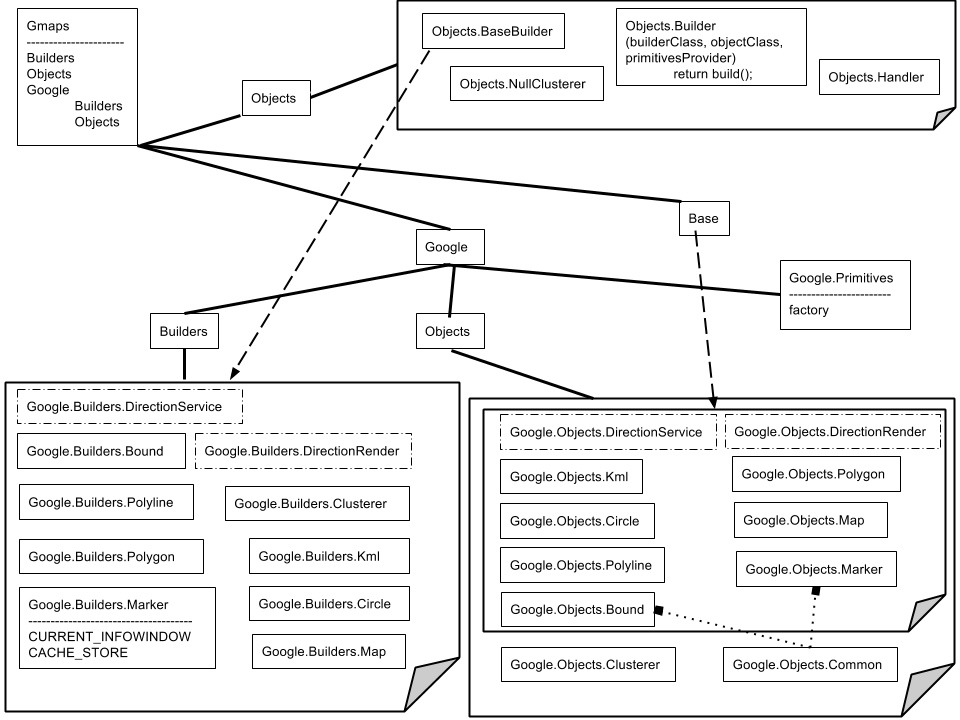
\includegraphics[scale=0.35]{images/novo_diagrama_de_heranca_google_maps_for_rails.png}
    \caption{Novo Diagrama de Herança Google-Maps-For-Rails}
    \label{fig:novo_diagrama_de_heranca_google_maps_for_rails}
  \end{center}  \
\end{figure}

Agora que acrescentamos estas quatro classes na gema adaptada, devemos adicionar no ‘‘\emph{Handler}'', 
novas funções para maminpular essas classes. E neste caso, inserimos as funçãoes ‘‘\emph{addDirection()}'' e 
‘‘\emph{calculate\_route()}'' que podem ser vistas no código \ref{lst:funcoes_adicionais_do_handler} que
será explicado logo a seguir.

\begin{itemize}

 \item Na linha ‘‘2'' é adicionado a função ‘‘\emph{addDirection}'' que recebe como parâmetro 
 ‘‘\emph{direction\_data}'', que possui o informações do local de origem e local de destino que são 
 obrigatórios para criar a direção, e ‘‘\emph{provider\_options}'' que pode conter as opções da forma
 como esse direção deve ser gerada. Essa função tem por objetivo criar as direções e colocá-las no mapas.
 
 \item Na linha ‘‘13'' é adicionado a função ‘‘\emph{calculate\_route}'' com o parâmetro 
 ‘‘\emph{direction\_data}'', que tem por principal objtivo fazer a requisição para o \emph{Google } de uma 
 possível direção entre o local de origem ao local de destino.
 
 \item Da linha ‘‘3'' a linha ‘‘10'' é o conteúdo da função ‘‘\emph{addDirection}'', onde se cria os
 atributos ‘‘\emph{direction\_service}'' e ‘‘\emph{direction\_render}'' para o ‘‘\emph{Handler}''. Para
 cada um deste atributos, é atribuido o seu respectivo objeto do \emph{Google Maps} com a chamada da função 
 ‘‘\emph{@\_builder(...)}''. Depois é feito a chamada da função ‘‘\emph{calulate\_route(...)}''
 para encontrar uma possível direção. E finalmente com o código 
 ‘‘\emph{@direction\_render.getServiceObject().setMap(@getMap())}'', a direção encontrada é colocado 
 no mapa.
 
 \item Da linha ‘‘13'' a linha ‘‘20'' é o conteúdo da função ‘‘\emph{calculate\_route(...)}'', onde 
 inicialmente é colocado em uma variável local o \emph{status Ok} de requisição que será utilizado
 para verificar se a requisição de direção foi feita com sucesso, e também é criada uma variável local 
 para o \emph{objeto DirectionRender} do \emph{Google Maps}. Em seguida, através da chamada da função 
 ‘‘\emph{route(...)}'' do \emph{objeto DirectionService}. Nesta função so parâmetros de entrada são,
 o local de origem e o local de destino, e como resposta se recebe o \emph{status} da requisição
 e o \emph{response}. Neste caso, \emph{response} pode ou não conter o caminho solução. Após a execução
 desta função, caso a resposta venha com o \emph{status Ok}, o \emph{objeto DirectionRender} recebe o
 caminho solução.
 
\end{itemize}

\lstinputlisting[ style=customCoffee, caption={Funções adicionais do Handler}, label={lst:funcoes_adicionais_do_handler}]
{codigos/funcoes_adicionais_do_handler.coffee}

Analisando as modificações, percebemos que somente inserimos 4 classes e 2 funções. Com isso podemos
perceber que as alterações que fizemos, não afetaram o funcionamento da gema, pois não foi
necessário mexer no código que já existia.

\section{Exemplo de uso de Google-Maps-for-Rails}
\label{section:exemplo_de_uso_de_google-maps-for-rails}

Esta seção tem o objetivo de mostrar a utilização da gema de exemplo ‘‘\emph{Google-Maps-for-Rails}'',
que adaptamos no tutorial, em um projeto do \emph{framework Ruby On Rails}.

Como exemplo de uso da gema ‘‘\emph{Google-Maps-for-Rails}'' adaptada, criamos o projeto 
‘‘\emph{\href{https://github.com/toshikomura/DiseasesMap}{DiseasesMap}}'' 
\footnote{DiseasesMap : \url{https://github.com/toshikomura/DiseasesMap}} que tem como objetivo representar 
a frequência de doenças no mapa do \emph{Google}, utilizando sobreposições. Até o momento de término deste
trabalho, essa função ainda não havia sido implementada, mas mesmo assim, fizemos o uso da
funcionalidade de direções, somente para exemplificar o uso da gema modificada.

Inicialmente fizemos a instalção e inclusão da gema adaptada no arquivo \emph{Gemfile} do projeto. Depois 
criamos uma estrutura básica de \emph{model/view/controller} de ‘‘\emph{locations}''. E para fazer o uso
da função de direções utilizamos o código \ref{lst:exemplo_coffeescript_que_cria_mapa_com_direcao},
explicado logo abaixo.

\lstinputlisting[ style=customCoffee, caption={Exemplo CoffeeScript que Cria Mapa com Direção}, label={lst:exemplo_coffeescript_que_cria_mapa_com_direcao}]
{codigos/DiseasesMap/app/assets/javascripts/locations.js.coffee}

\begin{itemize}

 \item Na linha ‘‘2'' é feita a preparação da estrtura de configuração do mapa com a chamada 
 ‘‘\emph{GMaps.build('Google')}'', sendo feita a criação do \emph{objeto Handler}, que é atribuida a 
 variável local ‘‘\emph{handler}'', juntamente com as outras configurações básicas que o mapa necessita.
 
 \item Na linha ‘‘3'' é feita a chamada de ‘‘\emph{handler.buildMap(...)}'' que tem como função, fazer a 
 criação do mapa a parir das configurações básicas já definidas. No caso, estas configurações básicas
 são definidas quando é feita a chamada de ‘‘\emph{GMaps.build('Google')}''. São passados como parâmetros
 as variáveis, ‘‘\emph{provider}'' que no exemplo está vazio, e internal que define o ‘‘\emph{id}'' do
 mapa como ‘‘\emph{map}''. Neste caso, o ‘‘\emph{id}'' serve para identificar o mapa a ser modificado.
 
 \item Na linha ‘‘7'' é criado uma \emph{function} determinada pelo símbolo ‘‘->''. Esta \emph{function}
 somente será executada depois que a função ‘‘\emph{handler.buildMap(...)}'' terminar, ou seja, quando a
 criação do mapa terminar.
 
 No exemplo do código essa função executa as seguintes operações:
 
  \subitem Na linha ‘‘8'' é feita a criação de um \emph{marker} com a chamada da função 
  ‘‘\emph{handler.addMarker(...)}'', sendo passado como parâmetro, a sua posição que no caso é (0,0) 
  definido ‘‘\emph{lat}'' e ‘‘\emph{lng}'', a sua imagem definida por ‘‘\emph{picture}'', e sua informação 
  definido por ‘‘\emph{infowindow}''.
 
  \subitem Na linha ‘‘17'' é feita a extensão de fronteiras incluindo o novo \emph{marker} com a chamada 
  da função ‘‘\emph{handler.bounds.extendWith(...)}'', sendo passado como parâmetro o \emph{marker} criado
  anteriormente.
 
  \subitem Na linha ‘‘19'' é feita a criação de direções com a chamada da função 
  ‘‘\emph{handler.addDirection(...)}''que incluimos no ‘‘\emph{Handler}'', sendo passado como parâmetro, um 
  local de origem definido por ‘‘\emph{ origin: ‘‘São Paulo''} '', e um local de destino definido por 
  ‘‘\emph{destination: ‘‘Curitiba''} ''.
 
\end{itemize}

E para mostrar o mapa na view de ‘‘\emph{locations}'' adicionamos o código mostrado em
\ref{lst:exemplo_locations_view_que_cria_mapa_com_direcao}
que é parte do código da \emph{view}, explicado logo a seguir.

\lstinputlisting[ style=customRubyHTML, caption={Exemplo Locations view que Cria Mapa com Direção}, label={lst:exemplo_locations_view_que_cria_mapa_com_direcao}]
{codigos/index_simplificado.html.erb}

\begin{itemize}

 \item Na linha ‘‘1'' com a \emph{tag} \emph{<h1>...</h1>} é definido como título principal da \emph{view} o
 texto ‘‘\emph{Listining locations}''.
 
 \item Os ‘‘\emph{...}'' indica que existe código, mas por simplificação na explicação, ele não fo mostrado.
 
 \item Da linha ‘‘3'' a ‘‘5'' é definido uma \emph{div} com ‘‘800px'' de largura. Dentro dessa \emph{div},
 é definido o local para a criação do mapa com ‘‘800px'' de largura e ‘‘400px'' de altura. No caso, o local 
 de criação do mapa, é referênciado pelo atributo \emph{id} que é o mesmo \emph{id} utilizado no código 
 \ref{lst:exemplo_coffeescript_que_cria_mapa_com_direcao} na linha ‘‘10''.  
 
\end{itemize}

Como resultado ao se acessar o \emph{index} de locations, obtemos como resultado a imagem
\ref{fig:caminho_entre_sao_paulo_e_curitiba}. Neste caso, a nossa gema adaptada com a nova funcionalidade
de direções, funcionou corretamente, pois o caminho mostrado é entre ‘‘São Paulo'' e ‘‘Curitiba'', como
requisitamos na linha ‘‘24'' do código \ref{lst:exemplo_coffeescript_que_cria_mapa_com_direcao}.

\begin{figure}[ht]
  \begin{center}       
    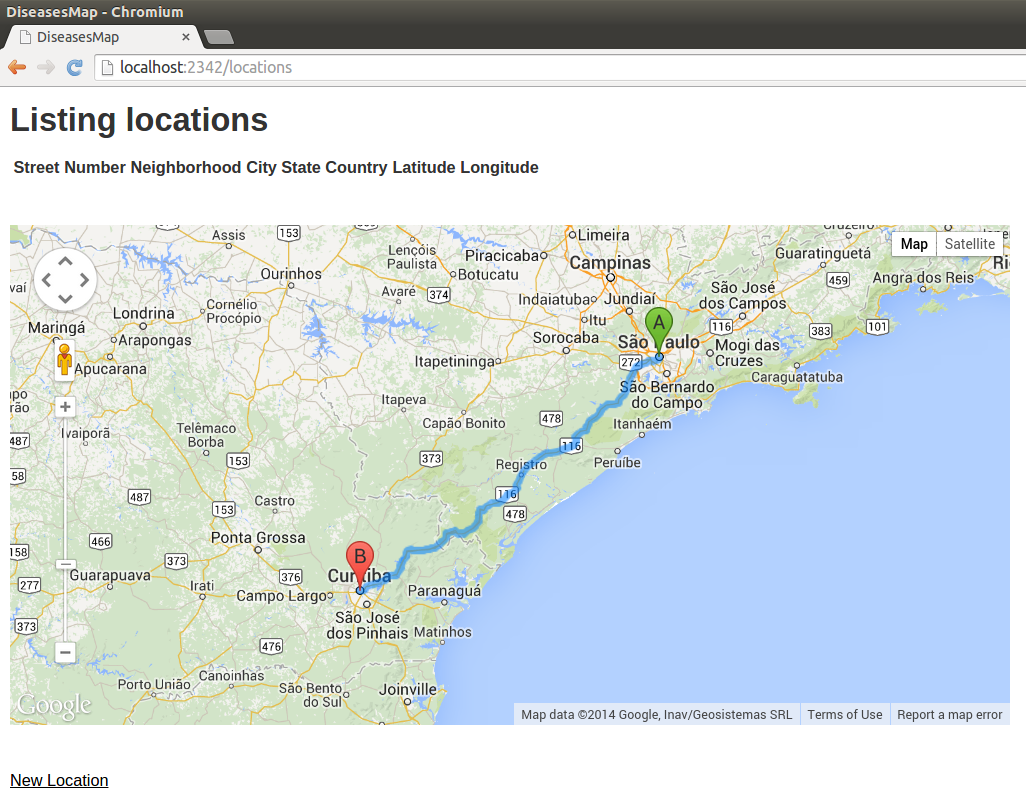
\includegraphics[scale=0.35]{images/caminho_entre_sao_paulo_e_curitiba.png}
    \caption{Caminho entre São Paulo e Curitiba}
    \label{fig:caminho_entre_sao_paulo_e_curitiba}
  \end{center}    
\end{figure}